\begin{figure}[!h]
    \centering
    \centering
    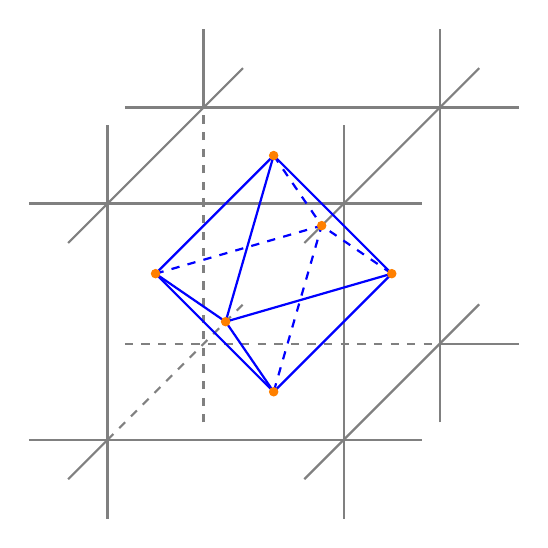
\begin{tikzpicture}
        % ---Z^3
        \draw[thick, gray] (-1, 0) -- (4, 0);
        \draw[thick, gray] (0, -1) -- (0, 4);
        \draw[thick, gray] (3, -1) -- (3, 4);
        \draw[thick, gray] (-1, 3) -- (4, 3);
        
        \draw[thick, gray, dashed] (0, 0) -- (1.72, 1.72);
        \draw[thick, gray] (-0.5, -0.5) -- (0, 0);
        \draw[thick, gray] (2.5, -0.5) -- (4.72, 1.72);
        \draw[thick, gray] (-0.5, 2.5) -- (1.72, 4.72);
        \draw[thick, gray] (2.5, 2.5) -- (4.72, 4.72);
        
        \draw[thick, gray, dashed] (1.22, 0.22) -- (1.22, 4.22);
        \draw[thick, gray] (1.22, 4.22) -- (1.22, 5.22);
        \draw[thick, gray, dashed] (0.22, 1.22) -- (4.22, 1.22);
        \draw[thick, gray] (4.22, 1.22) -- (5.22, 1.22);
        \draw[thick, gray] (4.22, 0.22) -- (4.22, 5.22);
        \draw[thick, gray] (0.22, 4.22) -- (5.22, 4.22);
        % \draw[thick] (0, 0) -- (3, 0);
        % \draw[thick] (0, 0) -- (0, 3);
        % \draw[thick] (3, 0) -- (3, 3);
        % \draw[thick] (0, 3) -- (3, 3);
        
        % \draw[thick, dashed] (0, 0) -- (1.22, 1.22);
        % \draw[thick] (3, 0) -- (4.22, 1.22);
        % \draw[thick] (0, 3) -- (1.22, 4.22);
        % \draw[thick] (3, 3) -- (4.22, 4.22);
        
        % \draw[thick, dashed] (1.22, 1.22) -- (1.22, 4.22);
        % \draw[thick, dashed] (1.22, 1.22) -- (4.22, 1.22);
        % \draw[thick] (4.22, 1.22) -- (4.22, 4.22);
        % \draw[thick] (1.22, 4.22) -- (4.22, 4.22);        
        
        % ---Z^3 dual
        
        \draw[blue, thick, dashed] (2.11, 3.61) -- (2.72, 2.72) -- (2.11, 0.61);
        \draw[blue, thick] (2.11, 3.61) -- (1.5, 1.5) -- (2.11, 0.61);
        \draw[blue, thick] (3.61, 2.11) -- (1.5, 1.5) -- (0.61, 2.11);
        \draw[blue, thick, dashed] (0.61, 2.11) -- (2.72, 2.72) -- (3.61, 2.11);
        \draw[blue, thick] (2.11, 0.61) -- (0.61, 2.11) -- (2.11, 3.61) -- (3.61, 2.11) -- (2.11, 0.61);
        
        \filldraw[orange] (1.5, 1.5) circle (1.5pt);
        \filldraw[orange] (2.72, 2.72) circle (1.5pt);
        \filldraw[orange] (2.11, 0.61) circle (1.5pt);
        \filldraw[orange] (2.11, 3.61) circle (1.5pt);
        \filldraw[orange] (0.61, 2.11) circle (1.5pt);
        \filldraw[orange] (3.61, 2.11) circle (1.5pt);
        
        % \draw[blue, thick] (1.5, 1.5) -- (2.72, 2.72);
        % \draw[blue, thick] (2.11, 0.61) -- (2.11, 3.61);
        % \draw[blue, thick] (0.61, 2.11) -- (3.61, 2.11);
        
        % \draw[cyan] (2.11, 3.61) -- (2.23, 4.03);
        % \draw[cyan] (2.11, 3.61) -- (1.81, 3.91);
        % \draw[cyan] (2.11, 3.61) -- (2.41, 3.91);
        % \draw[cyan] (2.11, 3.61) -- (1.99, 3.79);
        % \draw[cyan] (2.11, 3.61) -- (1.71, 3.61);
        % \draw[cyan] (2.11, 3.61) -- (2.51, 3.61);
        % \draw[cyan] (2.11, 3.61) -- (2.52, 4.02);
        % \draw[cyan] (2.11, 3.61) -- (1.70, 3.20);
        
    \end{tikzpicture}
    \caption{A $2 \times 2$ section of the simple cubic lattice (gray) and its dual (orange, blue)}
    \label{fig:z3_dual}
\end{figure}